\documentclass[pdftex,a4paper,14pt,english,russian]{extarticle}

\usepackage[top=2cm,bottom=27mm,left=3cm,right=18mm]{geometry}
\usepackage[T2A]{fontenc}
\usepackage[utf8]{inputenc}
\usepackage[english,russian]{babel}
\usepackage[pdftex]{hyperref}
\usepackage{indentfirst}
\usepackage[pdftex]{graphicx}
\usepackage{amsmath}
\usepackage{amssymb}
\usepackage{ragged2e}
\usepackage{multirow}
\usepackage{algorithmic}
\usepackage[boxed]{algorithm}
\usepackage{tabularx}
\usepackage{xtab}
\usepackage{subfig}
\usepackage{hyphenat}
\usepackage{setspace}
\usepackage{fancyhdr}
\usepackage{lastpage}

\pagestyle{fancyplain}
\fancyhf{}
\renewcommand{\headrulewidth}{0pt}
\rfoot{\fancyplain{}{\thepage}}

\linespread{1.15}
\floatname{algorithm}{Алгоритм}

\addto\captionsrussian{\renewcommand{\contentsname}{СОДЕРЖАНИЕ}}

\numberwithin{equation}{section}

% new commands
\newcommand\sign[1]{sign(#1)}
\newcommand{\todobiography}{insert biography here}

\begin{document}

\section*{Аннотация}
\thispagestyle{empty}

\begin{center}
  \begin{minipage}{0.8\textwidth}
    на дипломный проект ``Поисковые алгоритмы с учетом поведения пользователя для повышения релевантности поиска'' студента УО ``Белорусский государственный университет информатики и радиоэлектроники'' Иванова А.С.
  \end{minipage}
\end{center}

Дипломный проект выполнен на 6 листах формата А1 с пояснительной запиской на 68 страницах (без приложений справочного или информационного характера). Пояснительная записка включает 6 глав, 10 рисунков, 18 литературных источников.

Темой дипломной работы является актуальная проблема информационного поиска --- ранжирование результатов и использование неявных отзывов от пользователей. Целью данного дипломного проекта является исследовательский проект, демонстрирующий набор алгоритмов, который можно использовать для улучшения релевантности поисковой программы. 

В первой главе дипломного проекта дается обзор предметной области и архитекутры, меры, показывающие производительность алгоритма.

Во второй главе рассматривается градиентный бустинг, как метод усиления простых классификаторов.

Третья глава посвящена логическим деревьям решения, слабым классификаторам, которые обладают высокой информативностью и репрезентативностью.

В четвертой главе рассмотрен алгоритм динамической байесовской сети для нахождения релевантности документов из логов сессий пользователей.

Пятая глава посвящена безопасности работы инженеров\hyp{}разработчиков на предприятии малого бизнеса Акавита.

В шестой главе приводится расчет сетевого графика, дается расчет экономического эффекта от использования разработки. 

Глава ``Зкалючение'' содержит краткие выводы по дипломному проекту.

\newpage

\section*{Реферат}
\thispagestyle{empty}

Дипломный проект выполнен на 6 листах формата А1 с пояснительной запиской на 67 страницах (без приложений справочного или информационного характера). Пояснительная записка включает 6 глав, 10 рисунков, 19 литературных источников.

\emph{Ключевые слова}: поисковые системы, машинное обучение, логические деревья, байесовские сети, бустинг, обучение с учителем.


Целью данного дипломного проекта является исследдовательский проект, показывающий возможности улучшения релевантности поисковых технологий. Был рассмотрен стек алгоритмов, который использует как неявные отзывы от пользователей, так и векторы признаков документов. В конечном итоге, проект может быть внедрен в поисковые системы для улучшения ранжирования. Пояснительная записка состоит из следующих частей:

\emph{Введение}: описана актуальность проблемы в информационном поиске;

\emph{Глава 1}: описана предметная область и архитектура системы и меры, показывающие стойкость алгоритма; предлагается решение проблемы на основе алгоритмов машинного обучения;

\emph{Глава 2}: рассмотрен метод машинного обучения с учителем, основанный на бустинге для задачи ранжирования;

\emph{Глава 3}: описананы логические алгоритмы и деревья решения, которые используются бустингом в качестве слабых классификаторов

\emph{Глава 4}: описан метод нахождения релевантности документов из пользовательских сессий, основанный на динамической байесовской сети

\emph{Глава 5}: рассмотрена безопасность инденеров-разработчиков в компании малого бизнеса Акавита

\emph{Глава 6}: приводится расчет сетевого графика и дается расчет экономического эффекта от использования программного средства;

\emph{Заключение}: содержит краткие выводы по дипломному проекту.

\newpage


\setcounter{page}{1}
\tableofcontents
\newpage

\sectioncentered*{Введение}
\addcontentsline{toc}{section}{Введение}

Целью данного дипломного проекта является разработка алгоритмов машинного обучения, которые позволяют улучшить выдачу поисковых систем. Кроме этого проект демонстрирует как можно использовать неявные пользовательские отзывы(логи сессий) для улучшения ранжирования. 

Поиск информации представляет собой процесс выявления в некотором множестве документов (текстов) всех тех, которые посвящены указанной теме (предмету), удовлетворяют заранее определенному условию поиска (запросу) или содержат необходимые (соответствующие информационной потребности) факты, сведения, данные.

Процесс поиска включает последовательность операций, направленных на сбор, обработку и предоставление информации.

В общем случае поиск информации состоит из четырех этапов:

\begin{itemize}
	\item определение (уточнение) информационной потребности и формулировка информационного запроса
	\item определение совокупности возможных держателей информационных массивов (источников)
	\item извлечение информации из выявленных информационных массивов;
	\item ознакомление с полученной информацией и оценка результатов поиска
\end{itemize}

Информационный поиск — большая междисциплинарная область науки, стоящая на пересечении когнитивной психологии, информатики, информационного дизайна, лингвистики, семиотики, и библиотечного дела.

Поиск информации — процесс выявления в массиве информации записей, удовлетворяющих заранее определенному условию поиска или запросу.

Информационный поиск рассматривает поиск информации в документах, поиск самих документов, извлечение метаданных из документов, поиск текста, изображений, видео и звука в локальных реляционных базах данных, в гипертекстовых базах данных таких, как Интернет и локальные интранет-системы.

Существует некоторая путаница, связанная с понятиями поиска данных, поиска документов, информационного поиска и текстового поиска. Тем не менее, каждое из этих направлений исследования обладает собственными методиками, практическими наработками и литературой.

В настоящее время информационный поиск — это бурно развивающаяся область науки, популярность которой обусловлено экспоненциальным ростом объемов информации, в частности в сети Интернет. Информационному поиску посвящена обширная литература и множество конференций.

В последнее время наблюдается бурное развитие интернета. Количество интернет порталов и сайтов растет с очень большой скоростью и сейчас практически невозможно найти нужную информацию без поисковых систем. В свою очередь, поисковые системы должны отфильтровать и отсортировать огромный объём данных, чтобы предоставить желаемую информацию. Данная задача называется задачей ранжирования. 

Обучение ранжированию — это класс задач машинного обучения с учителем, заключающихся в автоматическом подборе ранжирующей модели по обучающей выборке, состоящей из множества списков и заданных частичных порядков на элементах внутри каждого списка. Частичный порядок обычно задаётся путём указания оценки для каждого элемента (например, «релевантен» или «не релевантен»; возможно использование и более, чем двух градаций). Цель ранжирующей модели — наилучшим образом (в некотором смысле) приблизить и обобщить способ ранжирования в обучающей выборке на новые данные. Это ещё довольно молодая, бурно развивающаяся область исследований, возникшая в 2000-е годы с появлением интереса в области информационного поиска к применению методов машинного обучения к задачам ранжирования.

Для любого алгоритма машинного обучения требуется обучающая выборка. Основной единицей обучения является пара документ-запрос и релевантность документа, данному запросу. Но, в зависимости от алгоритма обучения используются три подхода: 

\begin{itemize}

	\item Поточечный подход. В поточечном подходе предполагается, что каждой паре запрос-документ поставлена в соответствие численная оценка. Задача обучения ранжированию сводится к построению регрессии: для каждой отдельной пары запрос-документ необходимо предсказать её оценку.

	\item Попарный подход. В попарном подходе обучение ранжированию сводится к построению бинарного классификатора, которому на вход поступают два документа, соответствующих одному и тому же запросу, и требуется определить, какой из них лучше.

	\item Списочный подход. Списочный подход заключается в построении модели, на вход которой поступают сразу все документы, соответствующие запросу, а на выходе получается их перестановка. Подгонка параметров модели осуществляется для прямой максимизации одной из перечисленных выше метрик ранжирования.

\end{itemize}

Для построения модели ранжирования, был выбран поточечный подход. В данном дипломном проекте модель ранжирования представляет собой градиентный бустинг на основе решающих деревьев. Для получения релевантности документов из поисковых сессий была применена динамическая байесова сеть

Задача обучения ранжированию на онове кликов нетривиальна. В ~\cite{joachims} было показано, что даже если документы в выдаче отсортированы в обратном порядке(от худшего к лучшему), пользователи будут сначало производить клики по документам, которые занимают первые места. Поэтому, недостаточно просто отсортировать все документы по количеству кликов. В всязи с этим разрабатываются спеуиальные математические модели, которые потом тренируются на обучающей выборке для нахождения релевантности документов.

\newpage
\section{Предметная область}

\subsection{Задача обучения с учителем}

Обучение с учителем — один из способов машинного обучения, в ходе которого испытуемая система принудительно обучается с помощью примеров «стимул-реакция». С точки зрения кибернетики, является одним из видов кибернетического эксперимента. Между входами и эталонными выходами (стимул-реакция) может существовать некоторая зависимость, но она не известна. Известна только конечная совокупность прецедентов — пар «стимул-реакция», называемая обучающей выборкой. На основе этих данных требуется восстановить зависимость (построить модель отношений стимул-реакция, пригодных для прогнозирования), то есть построить алгоритм, способный для любого объекта выдать достаточно точный ответ. Для измерения точности ответов, так же как и в обучении на примерах, может вводиться функционал качества.

Пусть $X$ - множество описаний объектов, $Y$ - множество допустимых ответов. Существует неизвестная целевая зависимость - отображение $y: X \implies Y$, значения которой известны только на обучающей выборке 

\begin{equation}
  X_m=((x_1,y_1),...,(x_m,y_m))
\end{equation}

Требуется построить алгоритм 
\begin{equation}
  a: X \implies Y
\end{equation}
который приближал бы неизвестную целевую зависимость как на элементах выборки, так и на всём множестве $X$. 

Говорят также, что алгоритм должен обладать способностью к обобщению эмпирических фактов, или выводить общее знание (закономерность, зависимость) из частных фактов (наблюдений, прецедентов).

Данная постановка является обобщением классических задач аппроксимации функций. В классической аппроксимации объектами являются действительные числа или векторы. В реальных прикладных задачах входные данные об объектах могуть быть неполными, неточными, неоднородными, нечисловыми. Эти особенности приводят к большому разнообразию методов обучения с учителем. 

Признаком называется отображение $f: X \implies D_f$, где $D_f$- множество допустимых значений признака. Если заданы признаки $f_1,...,f_n$, то вектор
\begin{equation}
  x=(f_1(x),...,f_n(x))
\end{equation}
называется признаковым описанием объекта $x \in X$. Признаковые описания допустимо отождествлять с самими объектами. При этом множество $X=D_f1 ... D_fn$ называют признаковым пространством. 

В зависимости от множества $D_f$ признаки делятся на типы:
\begin{itemize}
  \item бинарныйы признак $D_f=(0,1)$
  \item номинальный признак $D_f$ - конечное множество
  \item порядковый признак $D_f$ - конечное упорядоченное множество
  \item количественный признак $D_f$ - множество действительных чисел.
\end{itemize}

\subsection{Задача обучения ранжированию}

\subsubsection{Классификация документов}

Классификация документов — одна из задач информационного поиска, заключающаяся в отнесении документа к одной из нескольких категорий на основании содержания документа.

Классификация может осуществляться полностью вручную, либо автоматически с помощью созданного вручную набора правил, либо автоматически с применением методов машинного обучения.

Следует отличать классификацию текстов от кластеризации, в последнем случае тексты также группируются по некоторым критериям, но заранее заданные категории отсутствуют.

Существует три подхода к задаче классификации текстов[1].

Классификация не всегда осуществляется с помощью компьютера. Например, в обычной библиотеке тематические рубрики присваиваются книгам вручную библиотекарем. Подобная ручная классификация дорога и неприменима в случаях, когда необходимо классифицировать большое количество документов с высокой скоростью.

Написании правил, по которым можно отнести текст к той или иной категории. Например, одно из таких правил может выглядеть следующим образом: "если текст содержит слова производная и уравнение, то отнести его к категории математика". Специалист, знакомый с предметной областью и обладающий навыком написания регулярных выражений, может составить ряд правил, которые затем автоматически применяются к поступающим документам для их классификации. Этот подход лучше предыдущего, поскольку процесс классификации автоматизируется и, следовательно, количество обрабатываемых документов практически не ограничено. Более того, построение правил вручную может дать лучшую точность классификации, чем при машинном обучении (см. ниже). Однако создание и поддержание правил в актуальном состоянии (например, если для классификации новостей используется имя действующего президента страны, соответствующее правило нужно время от времени изменять) требует постоянных усилий специалиста.

Третий подход основывается на машинном обучении. В этом подходе набор правил или, более обще, критерий принятия решения текстового классификатора, вычисляется автоматически из обучающих данных (другими словами, производится обучение классификатора). Обучающие данные — это некоторое количество хороших образцов документов из каждого класса. В машинном обучении сохраняется необходимость ручной разметки (термин разметка означает процесс приписывания класса документу). Но разметка является более простой задачей, чем написание правил. Кроме того, разметка может быть произведена в обычном режиме использования системы. Например, в программе электронной почты может существовать возможность помечать письма как спам, тем самым формируя обучающее множество для классификатора — фильтра нежелательных сообщений. Таким образом, классификация текстов, основанная на машинном обучении, является примером обучения с учителем, где в роли учителя выступает человек, задающий набор классов и размечающий обучающее множество.


\emph{Постановка задачи}.

Имеется множество категорий (классов, меток) $\mathfrak{C} = \{ c_1, ... , c_{ \left| \mathfrak{C} \right| } \}$.

Имеется множество документов $\mathfrak{D} = \{ d_1, ... , d_{ \left| \mathfrak{D} \right| } \}$.

Неизвестная целевая функция $\phi\colon \mathfrak{C} \times \mathfrak{D} \rightarrow \{ 0, 1 \}$.

Необходимо построить классификатор $\phi^\prime$ , максимально близкий к $\phi$.

Имеется некоторая начальная коллекция размеченных документов $\mathfrak{R} \subset \mathfrak{C} \times \mathfrak{D}$, для которых известны значения $\phi$. Обычно её делят на «обучающую» и «проверочную» части. Первая используется для обучения классификатора, вторая — для независимой проверки качества его работы.

Классификатор может выдавать точный ответ $\phi^\prime\colon \mathfrak{C} \times \mathfrak{D} \rightarrow \{ 0, 1 \}$ или степень подобия $\phi^\prime\colon \mathfrak{C} \times \mathfrak{D} \rightarrow [ 0, 1 ]$.

\emph{Этапы обработки}

\begin{itemize}

  \item Индексация документов. Построение некоторой числовой модели текста, например в виде многомерного вектора слов и их веса в документе. Уменьшение размерности модели.

  \item Построение и обучение классификатора. Могут использоваться различные методы машинного обучения: решающие деревья, наивный байесовский классификатор, нейронные сети, метод опорных векторов и др.

  \item Оценка качества классификации. Можно оценивать по критериям полноты, точности, сравнивать классификаторы по специальным тестовым наборам. 
\end{itemize}

\subsubsection{Ранжирование}

Обучение ранжированию — это класс задач машинного обучения с учителем, заключающихся в автоматическом подборе ранжирующей модели по обучающей выборке, состоящей из множества списков и заданных частичных порядков на элементах внутри каждого списка. Частичный порядок обычно задаётся путём указания оценки для каждого элемента (например, «релевантен» или «не релевантен»; возможно использование и более, чем двух градаций). Цель ранжирующей модели — наилучшим образом (в некотором смысле) приблизить и обобщить способ ранжирования в обучающей выборке на новые данные.

Применительно к поисковым системам, каждый список представляет собой набор документов, удовлетворяющих некоторому поисковому запросу.

Обучающая выборка состоит из выборки поисковых запросов, подмножества документов, им отвечающим, и оценок релевантности каждого документа запросу. Они могут быть подготовлены как вручную, специально натренированными людьми (оценщиками качества поиска или асессорами), так и автоматически, на основе анализа пользовательских кликов или таких средств поисковых систем, как система SearchWiki поисковой системы Google.

Задача улучшения ранжирования с использованием моделей поведения пользователей актуальна сейчас. Количество интернет документов и сайтов растет с оченьь большой скоростью, потребности пользователей меняются также очень быстро. Это ведет к быстрой смене релевантности документов, и ассессорам очень трудно проследить тенденции пользователей. Данная проблема имеет решение. Можно использовать неявную информацию о пользователях т.е. логи их поисковых запросов и кликов. Но правильное использование данной информации нетривиальная задача. Как показал ~\cite{joachims}, даже если документы отсортированы в обратном по релевантности порядке, пользователи всё равно будут нажимать на документы, которые стоят на первых местах.

Для решения данной проблемы строится математическая модель, которая обучается на тренеровачных данных. Было предложено ~\cite{ctr_improving1} добавить пользовательские данные, такие как количество кликов по URL, время проведения на странице, и т.д. в вектор признаков. 
Кроме этого, были предложены модели кликов ~\cite{ctr_improving2}, ~\cite{ccm}. В данном дипломном проекте рассматривается модель кликов, основанная на динамической байесовской сети ~\cite{dbn}.

\subsubsection{ Метрики качества ранжирования}

Существует несколько метрик, по которым оценивают и сравнивают качество работы алгоритмов ранжирования на выборке с асессорными оценками. Часто параметры ранжирующей модели стремятся подогнать так, чтобы максимизировать значение одной из этих метрик.

Примеры метрик:

\begin{itemize}
  \item Нормальная совокупная оценка(NDCG)
  \item Точность
  \item MAP
\end{itemize}

\subsubsection{Нормальная совокупная оценка}

Нормальная совокупная оценка используется для оценивания алгоритмов ранжирования. Данный вид оценки учитывает на только релевантность документа запросу, но также и его позицию в выдаче. Поэтому она достаточно точно отражает работу алгоритма.

Согласно ~\cite{ndcg_book} данная оценка вычисляется на основе Discounted Cumulative Gain. 

Discounted Cumulative Gain:

\begin{equation}
	DCG_p=\sum_{i=1}^{p}\frac{2^{{rel}_i}-1}{\log_2(i+1)}
\end{equation}

где ${rel}_i$ релевантность i-того документа, на позиции i. 

Т.к. количество ответов в запросе варьируется, то лучше считать нормализованныую общую оценку :

\begin{equation}
	{nDCG}_p=\frac{{DCG}_p}{{IDCG}_p}
\end{equation}

где ${{IDCG}_p}$ оценкка, вычисленная с выдачей, отсортированной по релевантности. При самом лучшем исходе, оцениваемая ввеличина ${{DCG}_p}$ равняется ${{IDCG}_p}$. 

\subsubsection{Точность}

В информационном поиске точность определяется как отношение числа релевантных документов, найденных информационной поисковой системой, к общему числу найденных документов:

\begin{equation}
  {Precision}=\frac{|D_{rel}\bigcap D_{retr}|}{|D_{rel}|}
\end{equation}

где $D_{rel}$ — это множество релевантных документов в базе, а $D_{retr}$ — множество документов, найденных системой. 

\subsection{Примененные алгоритмы}

В данном проекте были применены следующие алгоритмы:

\begin{itemize}
	\item Градиентный бустинг на основе слабых классификаторов для многослассовой задачи
	\item В качестве слабых классификаторов были использованы деревья решений
	\item В качестве целей(релевантностей документов для обучающей выборки) были использованы значения, найденные из логов пользователей с использованием динамимечкой байесовской сети
	\item Полученный алгоритм был оценен с помощью метрик NDCG, AUC, MAP.
\end{itemize}

\begin{figure}
  \centering
  \includegraphics[height=130mm]{images/architecture.png}
  \caption{Схематическое изображение системы\label{architecture}}
\end{figure}

Для ранжирования результатов был выбран градиентный бустинг с решающими деревьями. Основной причиной выбора стало то, что этот алгоритм работает не хуже, а иногда лучше ~\cite{cart_estimation_book} таких алгоритмов как метод опорных векторов и нейронная сеть. Кроме этого, градиентный бустинг с решающими деревьями обладает хорошей информативностью и слабым эффектом переобучения. ~\cite{cart_estimation_book}

Особенностью построения системы является то, что для хорошего рейтинга обучения необходимо достаточно большое количество данных и соответственно мощностей, чтобы вычислить эти данные. 

Структурная схема архитектуры приведена на рисунке ~\ref{architecture}

Данный дипломный проект демонстрирует построение алгоритма ранжирования использую современные технологии. Была продемонстрирована возможность использования действий пользователей для улучшения ранжирования. Также, централльный алгоритм обучения построен на основе деревьев, что позволяет построить схематический вид и интерпретировать результаты в вид, понятный для людей. 

Кроме этого, данный алгоритм позволяет построить диаграмму признаков и показать их информативность. Это позволяет оставить только те признаки, которые имеют информативность. Также можно проводить новые исследования и составлять алгоритмы для получения наилучшего вектора признаков(с наибольшей информативностью по признакам).

Задача информационного поиска специфична еще и тем, что обычные меры оценок не подходят. На рисунке ~\ref{feature-importance-picture} представлены информативности основных атрибутов, используемых для обучения алгоритма. Как видим, почти все они имеют одно и тоже значение, что делает задачу поиска довольно трудной.

\begin{figure}[h]
  \centering
  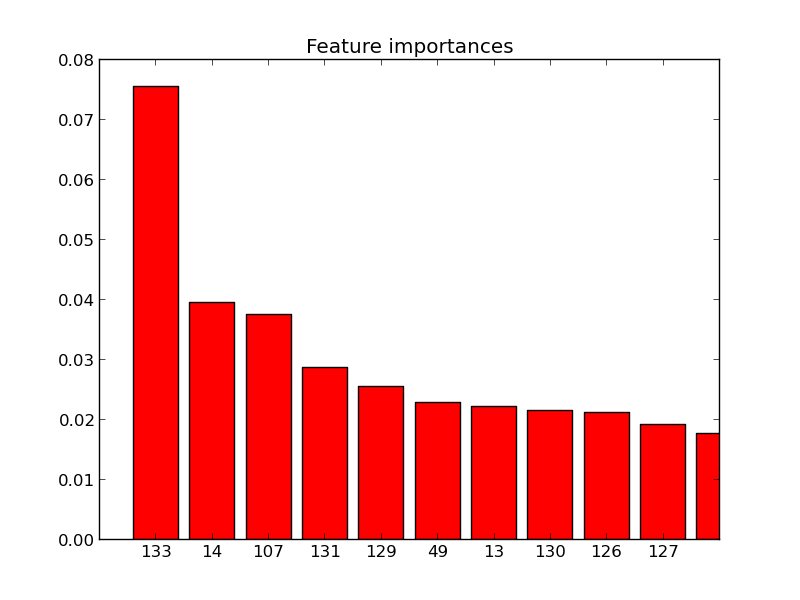
\includegraphics[width=1.0\textwidth]{images/feature_importance.png}
  \caption{Распределение  информативности образов\label{feature-importance-picture}}
\end{figure}



На рисунке ~\ref{precision-picture} приведен график зависимости точности от количества деревьев в сильном классификаторе:

\begin{figure}[h]
  \centering
  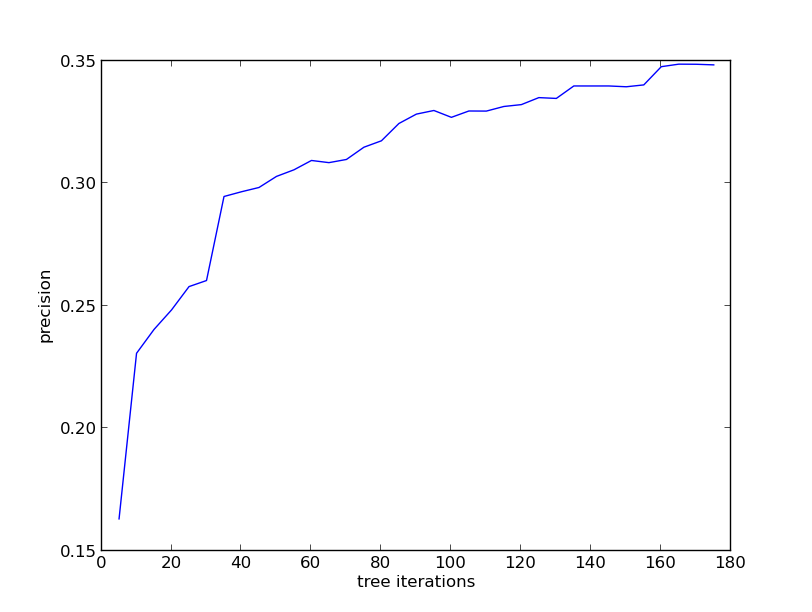
\includegraphics[width=1.0\textwidth]{images/precision_trees.png}
  \caption{График зависимости точности от количества слабых классификаторов в градиентном бустинге\label{precision-picture}}
\end{figure}

На рисунке ~\ref{ndcg-picture} приведен график зависимости нормализованной общей оценки от количества классификаторов в алгоритме бустинга. 

Как видим, с учеливением количества классификаторов растет и нормализованная общая оценка. При этом, в алгоритма бустинга не наблюдается переобучения. Поэтому данный алгоритм подходит для задачи ранжирования.

\begin{figure}[h]
  \centering
  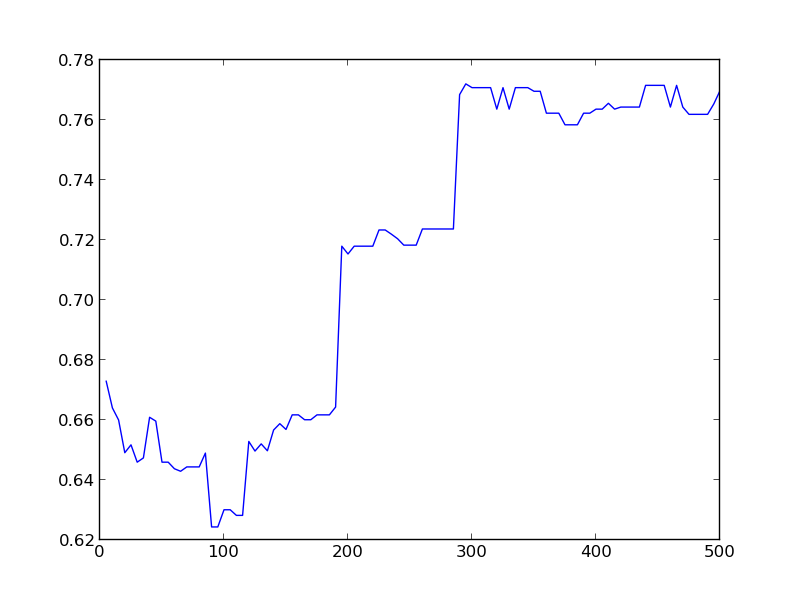
\includegraphics[width=1.0\textwidth]{images/ndcg_result1.png}
  \caption{График зависимости нормализованной общей оценки от количества слабых классификаторов\label{ndcg_result1}}
\end{figure}


\section{Композиции алгоритмов. Градиентный бустинг}

При решении сложных задач классификации, регрессии, прогнозирования часто оказывается, что ни один из алгоритмов не обеспечивает желаемого качества восстановления зависимости. В таких случаях имеет смысл строить композиции алгоритмов, в которых ошибки отдельных алгоритмов взаимно компенсируются. Наиболее известные примеры композиций — простое и взвешенное голосование. 

\subsection{Композиция алгоритмов}
Введем множество объектов $X$ и множество ответо $Y$. Наряду с этими множествами, введем вспомогательное множество $R$, называемое пространством оценок. Рассматриваются алгоритмы, имеющие вид суперпозиции $a(x)=C(b(x))$, где функция $b: X \to R$ называется алгоритмическим оператором, функция $C: R \to Y$ - решающее правило. 

Многие алгоритмы классификации имеют именно такую структуру: сначала вычисляются оценки принадлежности объекта классам, затем решающее правило переводит эти оценки в номер класса. Значением оценки $b(x)$ может быть вероятность принадлежности объекта x классу, расстояние от объекта до разделяющей поверхности, степень уверенности классификации и т.п.

Введем полное определение классификатора, на основе модели композиции. Композицией $T$ алгоритмов $a_t(x)= C(b_t(x)), t=1,\dotsc,T$ называется суперпозиция алгоритмических операторов $b_t: X \to R$, корректирующей операции  $F: R^T \to R$ и решающего правила $C: R \to Y$:


\begin{equation}
	a(x) = C(F(b_1(x),\dotsc,b_T(x))), x \in X
\end{equation}

Алгоритмы $a_t$, а иногда и операторы $bt$ , называют базовыми алгоритмами. 
Суперпозиции вида $F(b_1,\dotsc, b_T)$ являются отображениями из $X$ в $R$, то есть, опять-таки, алгоритмическими операторами. Это позволяет строить иерархические композиции, применяя определение 1.1 рекурсивно.

Пространство оценок $R$ вводится для того, чтобы расширить множество допустимых корректирующих операций. Можно было бы определить корректирующую операцию и как отображение $F: Y^T \to Y$ , то есть комбинировать непосредственно ответы базовых алгоритмов. Однако в задачах классификации, когда множество $Y$ конечно, число «разумных» корректирующих операций такого вида невелико, что ограничивает возможность оптимизации $F$ под конкретную задачу \todobiography. Если же ком бинировать ответы алгоритмических операторов, то операция $F$ получает на входе оценки принадлежности объекта классам — более точную информацию, не огрублённую решающим правилом.

\subsection{Взвешанное голосование}

Корректирующая операция $F$ может иметь параметры, настраиваемые по обучающей выборке, наряду с параметрами базовых алгоритмов. Например, в линейной комбинации настраиваются веса $at$ базовых алгоритмов:

\begin{equation}
	b(x)=F(b_1(x), \dotsc ,b_T(x)) = \sum_{t=1}^{T} a_tb_t(x),  x \in X,  a_t \in R
\end{equation}

Если веса $a_t$ неотрицательны и нормированы, $\sum_{t=1}^{T} a_t =1$ , то композицию (1.2) называют выпуклой комбинацией базовых алгоритмов. Естественно предполагать, что вес $a_t$ тем больше, чем выше качество базового алгоритма $b_t$.

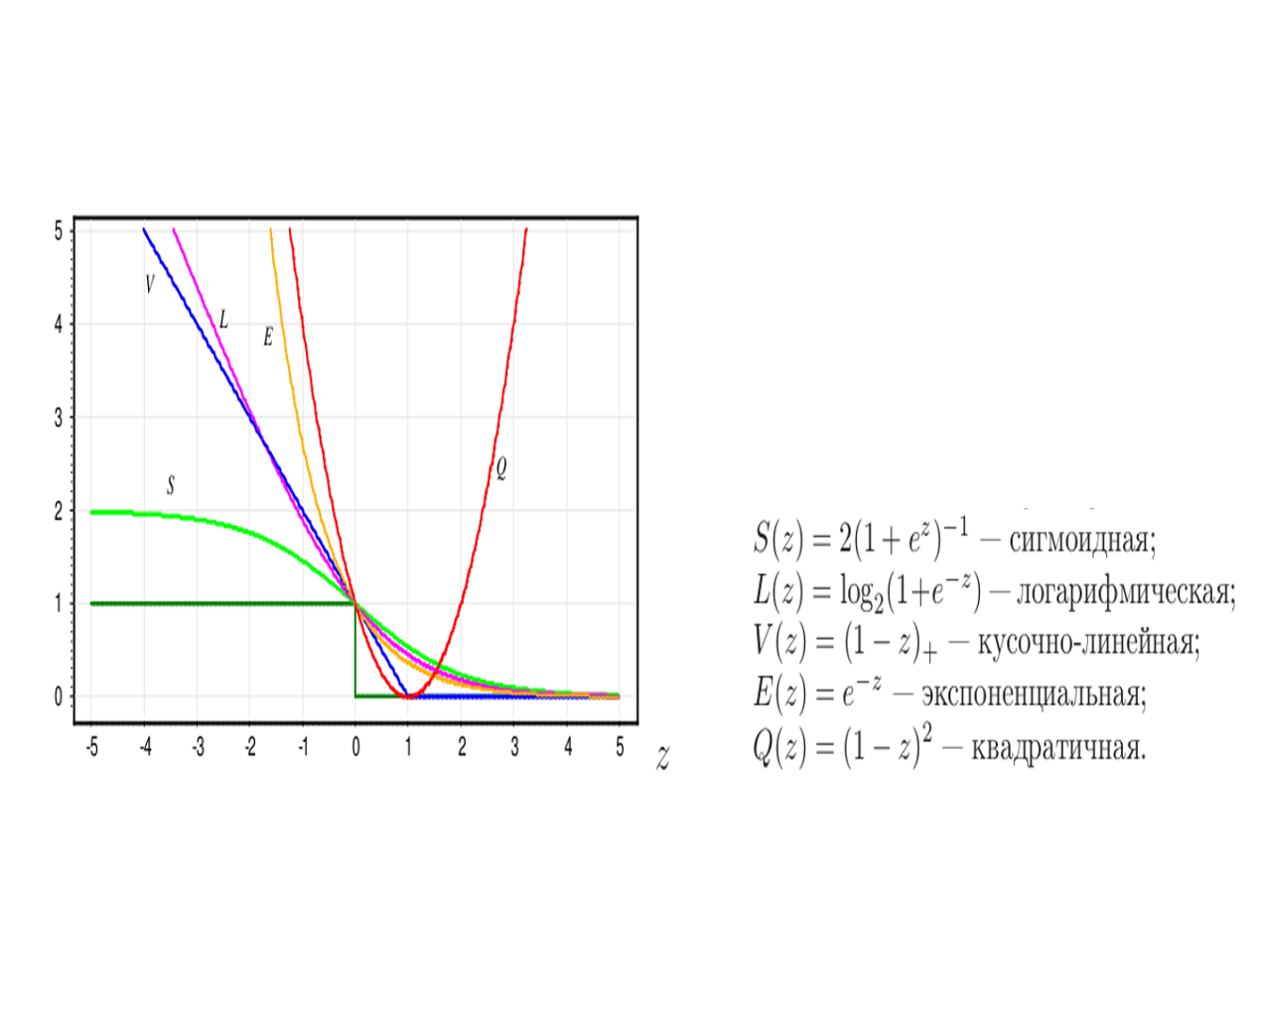
\includegraphics[width=0.9\textwidth]{images/upper_approximations.png}

\subsection{Бустинг}

Построение бустинга лучше всего рассматривать на задаче для двух классов ${-1,1}$, а потом обобщить на общий случай, для множества классов $M$. Пусть есть двух классовая задача $Y={-1,+1}$. Допустим, что решающее правило фиксировано, $C(b) = sign(b)$, базовые алгоритмы возвращают ответы $-1,0,+1$. Ответ $b_t(x) = 0$ означает, что базовый алгоритм $b_t$ отказывается от классификации объекта $x$, и ответ $b_t(x)$ не учитывается в композиции.
Искомая алгоритмическая композиция имеет вид:
\begin{equation}
	a(x)=C(F(b_1(x),\dotsc,b_T(x)))=sign(\sum_{t=1}^{T} a_tb_t(x)), x \in X
\end{equation}

Определим функционал качества композиции как число ошибок, допускаемых
ею на обучающей выборке:
\begin{equation}
	Q_T=\sum_{t=1}^{l} y_i\sum_{t=1}^{T} a_tb_t < 0]
\end{equation}

Напрямую, оптимизировать такой функционал очень сложно, поэтому заменим его на оценку сверху:
\begin{equation}
	Q_T=min_{\beta_m,\gamma_m}\sum_{i=1}^{N}L(y_i,\sum_{m=1}^{M}\beta_m b(x_i;\gamma_m)))
\end{equation}
В качестве функции потерь $L(y_i,f_m(x;\gamma)$ могут выступать функции, приведенные на рисунке 1.
Общий алгоритм бустинга:

\begin{algorithm}
  \caption{Общий алгоритм бустинга}
  \label{overall-boosting-algorithm}
  \begin{enumerate}
  \item Инициализировать переменные $f_0(x)=0$
  \item Для каждого шага $m=1,2 .. M$:
    \begin{enumerate}
      \item Вычисляем $(\beta_m,\gamma_m)=arg \min_{\beta,\gamma} \sum_{i=1}^{N}L(y_i,f_{m-1}(x_i)+\beta b(x_i;\gamma))$
      \item $f_m(x)=f_{m-1}(x)+\beta_m b(x;\gamma_m)$
    \end{enumerate}
  \end{enumerate}
\end{algorithm}



\begin{algorithm}
  \caption{Градиентный бустинг для многоклассовой классификации}
  \label{gradient-boosting-algorithm}
  \begin{enumerate}
  \item Инициализировать переменные $f_0(x)=0, k=1,2,...,K$
  \item Для каждого шага $m=1,2 .. M$:
    \begin{enumerate}
      \item Вычислить:
      \begin{equation}
      	p_k(x)=\frac{e^{f_k(x)}}{\sum_{l=1}^{K}e^{f_l(x)}}, k=1,2,...,K
      \end{equation}
      \item Для k = 1 до K:
      \begin{enumerate}
      	\item $r_{ikm}=y_{ik}-p_k(x_i), i=1,2,...,N$, где $y_{ik}=1$ если $y_i$ принадлежит классу $k$, иначе 0.
      	\item Для множества пар $(x_i,r_ikm)$ построить решающее дерево. С конечными регионами: $R_{jkm}, j=1,2,...,J_m$
      	\item $\gamma_{jkm}=\frac{K-1}{K}\frac{\sum_{x_i\in R_{jkm}}r_{ikm}}{\sum_{x_i\in R_{jkm}}|r_{ikm}|(1-|r_{ikm}|})$
      	\item Обновить $f_{km}=f_{k,m-1}(x)+\sum_{j=1}^{J_m}\gamma_{jkm}I(x\in R_{jkm}$
      \end{enumerate}
    \end{enumerate}
    \item Выход: $f_k=f_{km}(x), k=1,2,...,K$
  \end{enumerate}
\end{algorithm}
\section{Логические алгоритмы. Решающие деревья}

\subsection{Введение}

Логическая закономерность в задачах классификации — легко интерпретируемое правило, выделяющее из обучающей выборки достаточно много объектов какого-то одного класса и практически не выделяющее объекты остальных классов. Логические закономерности являются элементарными «строительными блоками» для широкого класса логических алгоритмов классификации, называемых также алгоритмами индукции правил 

В логических алгоритмах классификации принцип в индуктивном выводе логических закономерностей или индукции правил. Пусть $\phi:X \implies {0;1}$ — некоторый предикат, определённый на множестве объектов $X$. Говорят, что предикат $\phi$ выделяет или покрывает объект $x$, если $\phi(x) = 1$. Предикат называют закономерностью, если он выделяет достаточно много объектов какого-то одного класса $c$, и практически не выделяет объекты других классов. 

Особую ценность представляют закономерности, которые описываются простой логической формулой. Их называют правилами (rules). Процесс поиска правил по выборке называют извлечением знаний из данных. К знаниям предъявляется особое требование — они должны быть интерпретируемы, то есть понятны людям. На практике логические закономерности часто ищут в виде конъюнкций небольшого числа элементарных высказываний. Именно в такой форме люди привыкли выражать свой житейский и профессиональный опыт.

Всякая закономерность классифицирует лишь некоторую часть объектов. Объединив определённое количество закономерностей в композицию, можно получить алгоритм, способный классифицировать любые объекты. Логическими алгоритмами классификации будем называть композиции легко интерпретируемых закономерностей. 

Общая задача звучит так:
Имеется пространство объектов $X$ и конечное множество имён классов $Y= {1,...,M}$. Целевая зависимость $y^{*}: X \implies Y$ известа только на объектах обучающей выборки $X_l=(x_i,y_i)$.  Требуется построить алгоритм классификации $\alpha: X \implies Y$, аппроксимирующий $y^{*}$ на всё множестве $X$.

\subsection{Информативность}

Эвристическое определение информативности. Интуитивно предикат $\phi$ тем более информативен, чем больше он покрывает объектов некоторого фиксированного «своего» класса сY по сравнению с объектами всех остальных «чужих» классов. Введём следующие обозначения:
$G_c$ - число объектов класса с в выборке $X_l$
$g_c(\phi)$ - из них число объектов, для которых выполняется условие $(\phi(х) = 1)$
$B_c$ - число объектов всех остальных классов $Y \setminus {c}$ в выборке $X_l$
$b_c(\phi)$ -  из них число объектов, для которых выполняется условие $\phi(х) = 1$.

Чем   больше   число   покрываемых объектов $(g+b)$ и чем меньше среди них ошибочных $b$, тем более информативен предикат $\phi$. И, наоборот, наименее интересны предикаты, которые либо покрывают слишком мало объектов, либо выделяют «свои» и «чужие» объекты примерно в той же пропорции, в которой они представлены во всей выборке, $b:g \sim B:G$.

Введём обозначение $E_c$ для доли ошибочно покрываемых «чужих» объектов, и $D_c$ для доли всех покрываемых объектов:

\begin{subequations}
\begin{align}
	E_c(\phi,X_l)=\frac{b_c(\phi)}{b_c(\phi)+g_c(\phi)} \\
	D_c(\phi,X_l)=\frac{b_c(\phi)+g_x(\phi)}{l}
\end{align}
\end{subequations}

Если $bс(\phi)=0$, то закономерность $\phi$ называется чистой или непротиворечивой.Если $b_c(\phi)>0$, то закономерность $\phi$ называется частичной.

В некоторых случаях имеет смысл ограничиваться поиском только чистых закономерностей. В частности, когда длина выборки мала или заранее известно, что данные практически не содержат шума. Такие прикладные задачи нередко встречаются на практике, например, классификация месторождений редких полезных ископаемых по данным геологоразведки.

Но чаще данные оказываются неполными и неточными. Таковы многие медицинские и экономические задачи (в частности, задача о выдаче кредитов). Для них незначительная доля ошибок $\epsilon$ на обучающей выборке вполне допустима. Кроме того, существуют способы построения корректных алгоритмов на основе частичных закономерностей, например, взвешенное голосование. В этих случаях сравнивать и отбирать предикаты приходится по двум критериям $(g,b)$ одновременно.

\subsection{Информационная энтропия}

Информационная энтропия — мера неопределённости или непредсказуемости информации, неопределённость появления какого-либо символа первичного алфавита. При отсутствии информационных потерь численно равна количеству информации на символ передаваемого сообщения.

Например, в последовательности букв, составляющих какое-либо предложение на русском языке, разные буквы появляются с разной частотой, поэтому неопределённость появления для некоторых букв меньше, чем для других. Если же учесть, что некоторые сочетания букв (в этом случае говорят об энтропии n-ого порядка, см. ниже) встречаются очень редко, то неопределённость уменьшается еще сильнее.

Для иллюстрации понятия информационной энтропии можно также прибегнуть к примеру из области термодинамической энтропии, получившему название демона Максвелла. Концепции информации и энтропии имеют глубокие связи друг с другом, но, несмотря на это, разработка теорий в статистической механике и теории информации заняла много лет, чтобы сделать их соответствующими друг другу.

Энтропия — это количество информации, приходящейся на одно элементарное сообщение источника, вырабатывающего статистически независимые сообщения.

Энтропийное определение информативности. Ещё один способ определения информативности вытекает из теории информации. Если имеются два исхода $w_0$ , $w_1$ с вероятностями $q_0$ и $q_1=1-q_0$, то количество информации, связанное с исходом $w_i$ , по определению равно $-\log_2 q_i$. Это математическое ожидание числа бит, необходимых для записи информации о реализации исходов $w_i$ при использовании оптимального (наиболее экономного) кодирования. Энтропия определяется как матожидание количества информации:

\begin{equation}
	H(q_0,q_1)=-q_0\log_2 q_0-q_1\log_2 q_1
\end{equation}

Будем считать появление объекта класса $c$ исходом $w_0$, а появление объекта любого другого класса исходом $w_1$. Тогда, подставляя вместо вероятностей частоты, можно оценить энтропию выборки $X_l$:

\begin{equation}
	H(P,N)=H(\frac{P}{P+N},\frac{N}{N+P})
\end{equation}

Допустим, стало известно, что предикат $\phi$ выделил $p$ объектов из $P$, принад-
лежащих классу $c$, и $n$ объектов из $N$, не принадлежащих классу $c$. Тогда энтропия выборки ${x\in X_l|\phi(x)=1}$ есть $H(p,n)$. Вероятность появления объекта из этой выборки оценивается как $\frac{p+n}{P+N}$. Аналогично, энтропия выборки ${x\in X_l|\phi(x)=0}$ есть $H(P-p,N-n)$, а вероятность появления объекта из неё оценивается как $\frac{P-p+N-n}{P+N}$. Таким образом, энтропия всей выборки после получения информации $\phi$ становится равна

\begin{equation}
	H_{\phi}(P,N,p,n)=\frac{p+n}{P+N}H(p,n) + \frac{P+N-p-n}{P+N}H(P-p,N-n)
\end{equation}

В итоге уменьшение энтропии составит:

\begin{equation}
	{IGain}_c(\phi,X_l)=H(P,N)-H(P,N,p,n)
\end{equation}

Это и есть информационный выигрыш (information gain) — количество информа-
ции об исходном делении выборки на два класса $c$ и $не c$, которое содержится
в предикате $\phi$. Таким образом, появляется ещё одно, альтернативное, определение
закономерности.

Несмотря на асимптотическую эквивалентность, значения $I_c$ и ${IGain}_c$ могут заметно отличаться при малых $n$ или $p$. Согласно таблице 1, критерий ${IGain}_c$ полагает, что «маломощная» закономерность $(n,p)=(0,5)$ лучше, чем «полное отсутствие закономерности» $(50,100)$, тогда как точный тест $I_c$ показывает противоположное. Иными словами, критерий IGain завышает информативность маломощных закономерностей. Ситуации малых $n$ или $p$ вовсе не экзотичны, они регулярно возникают при построении решающих списков и деревьев. Точный критерий может давать в этих ситуациях ощутимые преимущества ~\cite{martin}. Однако на практике чаще используется энтропийный критерий, поскольку он проще вычисляется.

Когда число классов превышает 3, приходится оценивать информативность не только таких предикатов, которые отделяют один класс от остальных, но и таких, которые отделяют некоторую группу классов от остальных.

Энтропийный критерий для случая большого числа классов:

\begin{equation}
	I(\phi,X_l)=\sum_{c\in Y}h(\frac{P_c}{l})-\frac{p}{l}\sum_{c\in Y}h(\frac{p_c}{p})-\frac{l-p}{l}\sum_{c\in Y}h(\frac{P_c-p_c}{l-p})
\end{equation}
\par
где введена функция $h(z)=-z\log_2 z$.

\subsection{Решающие деревья.}

Решающее дерево — это логический алгоритм классификации, основанный на поиске конъюнктивных закономерностей. При синтезе дерева все конъюнкции строятся одновременно. Деревом называется конечный связный граф с множеством вершин $V$ , не содержащий циклов и имеющий выделенную вершину $v_0 \in V$ , в которую не входит ни одно ребро. Эта вершина называется корнем дерева. Вершина, не имеющая выходящих рёбер, называется терминальной или листом. Остальные вершины называются внутренними. Дерево называется бинарным, если из любой его внутренней вершины выходит ровно два ребра. Выходящие рёбра связывают каждую внутреннюю вершину $v$ с левой дочерней вершиной $L_v$ и $с$ правой дочерней вершиной $R_v$.

Деревья классификации - это метод, позволяющий предсказывать принадлежность наблюдений или объектов к тому или иному классу категориальной зависимой переменной в зависимости от соответствующих значений одной или нескольких предикторных переменных. Построение деревьев классификации - один из наиболее важных методов, используемых при проведении добычи данных.

Цель построения деревьев классификации заключается в предсказании (или объяснении) значений категориальной зависимой переменной, и поэтому используемые методы тесно связаны с более традиционными методами Дискриминантного анализа, Кластерного анализа, Непараметрической статистики и Нелинейного оценивания. Широкая сфера применимости деревьев классификации делает их весьма привлекательным инструментом анализа данных.

\subsection{Детали реализации}

В данном дипломном проекте были использованы классифицирующие деревья решений~\cite{cart_book}. Дальше будет описан алгоритм построения таких деревьев для задачи ранжирования.

Для поиска атрибутов с максимальной информативностью была использована энтропия. Сам алгоритм разрабатывался с целью использования как слабого классифицирующего алгоритма в градиентном бустинге.

\begin{figure}
  \centering
  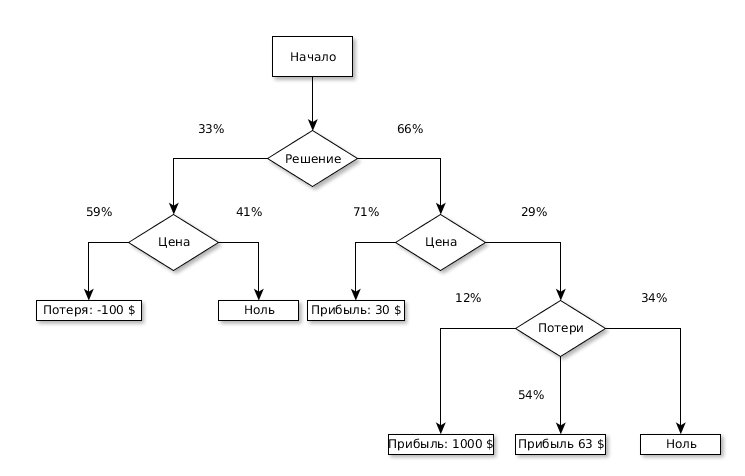
\includegraphics[width=1.0\textwidth]{images/decision_tree_new.jpg}
  \caption{Пример решающего дерева\label{decision_tree_schema}}
\end{figure}

Структурна схема алгоритма приведена на рисунке ~\ref{decision_tree_schema}.

Сам алгоритм приведен на ~\ref{decision-tree-algorithm}:

\begin{algorithm}
  \caption{Построение решающего дерева}
  \label{decision-tree-algorithm}
  \begin{enumerate}
  \item Загрузить обучающую выборку $(x_i,y_i)$
  \item Задать переменные $max_tree_depth,min_subset_length$
  \item Пока выполняется критерий
  	\begin{enumerate}
  		\item Выбрать атрибут из вектора $x_i$
  		\item Посчитать энтропию $H(Y)$
  		\item для каждого элемента обучающей выборки
  		\begin{enumerate}
  			\item Посчитать энтропию атрибута при $H(Y|X_i)$
  		\end{enumerate}
  		\item Взять атрибут $x_{ij}$ с максимальной информативностью.
  		\item Поделить выборку на 2.
  			\begin{subequations}
  			\begin{align}
  				R_1(j,s)={X|X_j < s} \\
  				R_2(j,s)={X|X_j > s}
  			\end{align}
  			\end{subequations}
  	\end{enumerate}
  \end{enumerate}
\end{algorithm}


Преимущества алгоритма:

\begin{itemize}
  \item Простота и интерпретируемость классификации. Алгоритм способен
не только классифицировать объект, но и выдать объяснение классификации
в терминах предметной области. Объяснение строится путём выписывания по-
следовательности условий, проверенных для данного объекта на пути от корня
дерева до листа $v$. Эти условия образуют конъюнкцию $K_v$ , то есть легко интер-
претируемое логическое правило.
  \item Не бывает отказов от классификации, в отличие от решающих списков.
  \item  Алгоритм очень прост для реализации и легко поддаётся различным усовершенствованиям. Можно использовать различные критерии ветвления и критерии останова, вводить редукцию, и т. д.
 \end{itemize}

Недостатки алгоритма:

\begin{itemize}
  \item Проблема получения оптимального дерева решений является NP-полной с точки зрения некоторых аспектов оптимальности даже для простых задач ~\cite{cart_optimal1} ~\cite{cart_optimal2}. Таким образом, практическое применение алгоритма деревьев решений основано на эвристических алгоритмах, таких как алгоритм «жадности», где единственно оптимальное решение выбирается локально в каждом узле. Такие алгоритмы не могут обеспечить оптимальность всего дерева в целом.
  \item Те, кто изучает метод дерева принятия решений, могут создавать слишком сложные конструкции, которые не достаточно полно представляют данные. Данная проблема называется проблемой «чрезмерной подгонки»~\cite{cart_optimal3} Для того, чтобы избежать данной проблемы, необходимо использовать Метод «регулирования глубины дерева».
  \item Существуют концепты, которые сложно понять из модели, так как модель описывает их сложным путем. Данное явление может быть вызвано проблемами XOR, четности или мультиплексарности. В этом случае мы имеем дело с непомерно большими деревьями. Существует несколько подходов решения данной проблемы, например, попытка изменить репрезентацию концепта в модели (составление новых суждений)~\cite{cart_optimal4}, или использование алгоритмов, которые более полно описывают и репрезентируют концепт (например, метод статистических отношений, индуктивная логика программирования).
  \item Для данных, которые включают категориальные переменные с большим набором уровней (закрытий), больший информационный вес присваивается тем атрибутам, которые имеют большее количество уровней.~\cite{cart_optimal5}
 \end{itemize}

В ходе разработки алгоритма, был построен алгоритм для решения задачи классификации с множеством классов. Т.к. данный алгоритм планируется использовать с градиентным бустингом, то редукция деревьев не была нужна. Максимальная глубина дерева составила 8. Кроме этого, все параметры вектора $x_i \in R$, поэтому при поиске наилушего атрибута приходилось пробегать по значению $x_{ij}$ для всей выборке. 

\newpage
\section{Динамическая байесова сеть}

Байесова сеть — графическая вероятностная модель, представляющая собой множество переменных и их вероятностных зависимостей. Например, байесова сеть может быть использована для вычисления вероятности того, чем болен пациент по наличию или отсутствию ряда симптомов, основываясь на данных о зависимости между симптомами и болезнями.

Формально, байесова сеть — это направленный ациклический граф, каждой вершине которого соответствует случайная переменная, а дуги графа кодируют отношения условной независимости между этими переменными. Вершины могут представлять переменные любых типов, быть взвешенными параметрами, скрытыми переменными или гипотезами. Существуют эффективные методы, которые используются для вычислений и обучения байесовых сетей. Если переменные байесовой сети являются дискретными случайными величинами, то такая сеть называется дискретной байесовой сетью. Байесовы сети, которые моделируют последовательности переменных, называют динамическими байесовыми сетями. Байесовы сети, в которых могут присутствовать как дискретные переменные, так и непрерывные, называются гибридными байесовыми сетями. 

\subsection{Определение}
Если дуга выходит из вершины $A$ в вершину $B$, то $A$ называют родителем $B$, а $B$ называют потомком $A$. Если из вершины $A$ существует ориентированный путь в другую вершину $B$, то $B$ называется потомком $A$, а $A$ называется предком $B$. Множество вершин-родителей вершины $V_i$ обозначим как $parents(V_i) = PA_i$.

Направленный ациклический граф G называется байесовой сетью для вероятностного распределения $P(v)$, заданного над множеством случайных переменных $V$, если каждой вершине графа поставлена в соответствие случайная переменная из $V$, а дуги в графе удовлетворяют условию (марковское условие ~\cite{m_chain}): любая переменная $V_i$ из $V$ должна быть условно независима от всех вершин, не являющихся ее потомками, если заданы (получили означивание, обусловлены) все ее прямые родители $PA_i$ в графе $G$, то есть $\forall V_i \in V$ справедливо: $P(v_i|pa_i,s) = P(v_i|pa_i)$, где $v_i$ — значение $V_i; S$ — множество всех вершин, не являющихся потомками $V_i$; $s$ — конфигурация $S$; $pa_i$ — конфигурация $PA_i$.

Тогда полное совместное распределение значений в вершинах можно удобно записать в виде декомпозиции (произведения) локальных распределений:

\begin{equation}
	P(V_1,...,V_n)=\prod_{i=1}^{n}P(V_i|parents(V_i))
\end{equation}

Если у вершины $V_i$ нет предков, то её локальное распределение вероятностей называют безусловным, иначе условным. Если вершина - случайная переменная получила означивание (например, в результате наблюдения), то такое означивание называют свидетельством. Если значение переменной было установлено извне (а не наблюдалось), то такое означивание называется вмешательством.

\subsection{Цепь маркова}
Цепь Маркова — последовательность случайных событий с конечным или счётным числом исходов, характеризующаяся тем, что при фиксированном настоящем будущее независимо от прошлого.

Процесс в каждый момент времени находится в одном из $n$ состояний. 
При этом, если он находится в состоянии с номером $i$, то он перейдет в состояние $j$ с вероятностью $p_{ij}$.
Матрицу $P=||p_{ij}||$ называют матрицей переходов.

На матрицу переходов накладываются следующие условия: 

\begin{subequations}
\begin{align}
  p_{ij}>0 \\
  \forall i \sum_j p_{i,j}=1
\end{align}
\end{subequations}

Такая матрица называется стохастической.

Марковскую цепь можно представить в виде графа, в котором вершины — это состояния процесса, а ребра — переходы между состояниями, и на ребре из $i$ в $j$ написана вероятность перехода из $i$ в $j$, то есть $p_{ij}$. 

Марковскую цепь в любой момент времени $t$ можно охарактеризовать вектором-строкой $c_t$ — распределением вероятностей по состояниям цепи ($c_{ti}$ — вероятность цепи в момент времени $t$ быть в состоянии $i$). 

Если $c_i$ — текущее распределение вероятностей, то можно узнать распределение на следующем шаге, умножив вектор на матрицу перехода: 

\begin{equation}
  c_{i+1}=c_i P
\end{equation}

Из ассоциативности произведения матриц следует, что для того, чтобы узнать распределение вероятностей через $t$ шагов, нужно умножить $c_i$ на матрицу перехода, возведённую в степень $t$: 

\begin{equation}
  c_{i+t}=c_i P_t
\end{equation}

Для марковской цепи иногда задают начальное распределение $c_0$, хотя во многих классах марковских цепей распределение по прошествии большого периода времени от него не зависит (такое распределение называют предельным). 

\subsection{EM - алгоритм}

EM-алгоритм (Expectation-maximization (EM) algorithm) — алгоритм, используемый в математической статистике для нахождения оценок максимального правдоподобия параметров вероятностных моделей, в случае, когда модель зависит от некоторых скрытых переменных. Каждая итерация алгоритма состоит из двух шагов. На E-шаге (expectation) вычисляется ожидаемое значение функции правдоподобия, при этом скрытые переменные рассматриваются как наблюдаемые. На M-шаге (maximization) вычисляется оценка максимального правдоподобия, таким образом увеличивается ожидаемое правдоподобие, вычисляемое на E-шаге. Затем это значение используется для E-шага на следующей итерации. Алгоритм выполняется до сходимости.

Пусть \textbf{X} — некоторые из значений наблюдаемых переменных, а \textbf{T} — скрытые переменные. Вместе \textbf{X} и \textbf{T} образуют полный набор данных. Вообще, \textbf{T} может быть некоторой подсказкой, которая облегчает решение проблемы в случае, если она известна. Например, если имеется смесь распределений, функция правдоподобия легко выражается через параметры отдельных распределений смеси.

Положим $p$, — плотность вероятности (в непрерывном случае) или функция вероятности (в дискретном случае) полного набора данных с параметрами $\theta: p(X,T|\theta)$. Эту функцию можно понимать как правдоподобие всей модели, если рассматривать её как функцию параметров $\theta$. Заметим, что условное распределение скрытой компоненты при некотором наблюдении и фиксированном наборе параметров может быть выражено так:

\begin{equation}
	P(T|X,\theta)=\frac{p(X|T,\theta)}{p(X|\theta)}=\frac{p(X|T,\theta)p(T|\theta)}{\int p(X|T,\theta)p(T|\theta)dT}
\end{equation}
\par
используя расширенную формулу Байеса и формулу полной вероятности. Таким образом, нам необходимо знать только распределение наблюдаемой компоненты при фиксированной скрытой $p(X|T,\theta)$ и вероятности скрытых данных $p(T|\theta)$.

EM-алгоритм итеративно улучшает начальную оценку $\theta_0$, вычисляя новые значения оценок $\theta_1$, $\theta_2$, и так далее. На каждом шаге переход к $\theta_{n+1}$, от $\theta_n$, выполняется следующим образом:

\begin{equation}
	\theta_{n+1}=arg \max_{\theta} Q(\theta)
\end{equation}
\par
где $Q(\theta)$ — матожидание логарифма правдоподобия. Другими словами, мы не можем сразу вычислить точное правдоподобие, но по известным данным ($X$) мы можем найти апостериорную оценку вероятностей для различных значений скрытых переменных $T$. Для каждого набора значений $T$ и параметров $\theta$ мы можем вычислить матожидание функции правдоподобия по данному набору $X$. Оно зависит от предыдущего значения $\theta$, потому что это значение влияет на вероятности скрытых переменных $T$.

$Q(\theta)$ вычисляется следующим образом:

\begin{equation}
	Q(\theta) = E_T[\log p(X,T|\theta)|X]
\end{equation}


\subsection{Алгоритм построения динамической байесовой сети}

Для решения задачи кликов, построим математичепскую модель. Будем предполагать, что пользователь просматривает документы последовательно сверху вниз, при этом производя клики на документы, которые его заинтересовали. Ввод нового запроса будем ассоциировать с новой сессией. Это довольно схоже с каскадной моделью кликов.~\cite{cascade_click_book}

Динамическая байесова сеть представляет из себя марковскую цепь, представленную на ~\ref{dbn-picture}. Это вероятностная модель, основанная на действиях пользователей. В ней рассматриваются сессии целиком. В этом случае для каждой сессии мы можем построить марковскую цепь. Для i-того документа имеем $C_i$ - клик пользователя на документ - наблюдаемый параметр, также набор скрытых переменных, которые описаны ниже.	

Данная модель определяется следующими параметрами(представленные ниже параметры могут принимать значения ${0;1}$): 
\begin{itemize}
	\item $A_i$ - привлекательность i-того документа для пользователя. 
	\item $E_i$ - параметр, определяющий посмотрел ли пользователь i-тый документ. 
	\item $S_i$ - удовлетворенность документом.
\end{itemize}

С учетом этого, мы можем записать полную вероятностную модель:

\begin{subequations}
\begin{align}
	A_i=1,E_i=1 \iff  C_i=1 \\
	P(A_i)=a_u \\
	P(S_i=1|C_i=1)=s_u \\
	C_i=0 \implies S_i=0 \\
	S_i=1 \implies E_{i+1}=0 \\
	P(E_{i+1}=1|E_i=1,S_i=0)=\gamma \\
	E_i=0 \implies E_{i+1}=0 
\end{align}
\end{subequations}

\begin{figure}
  \centering
  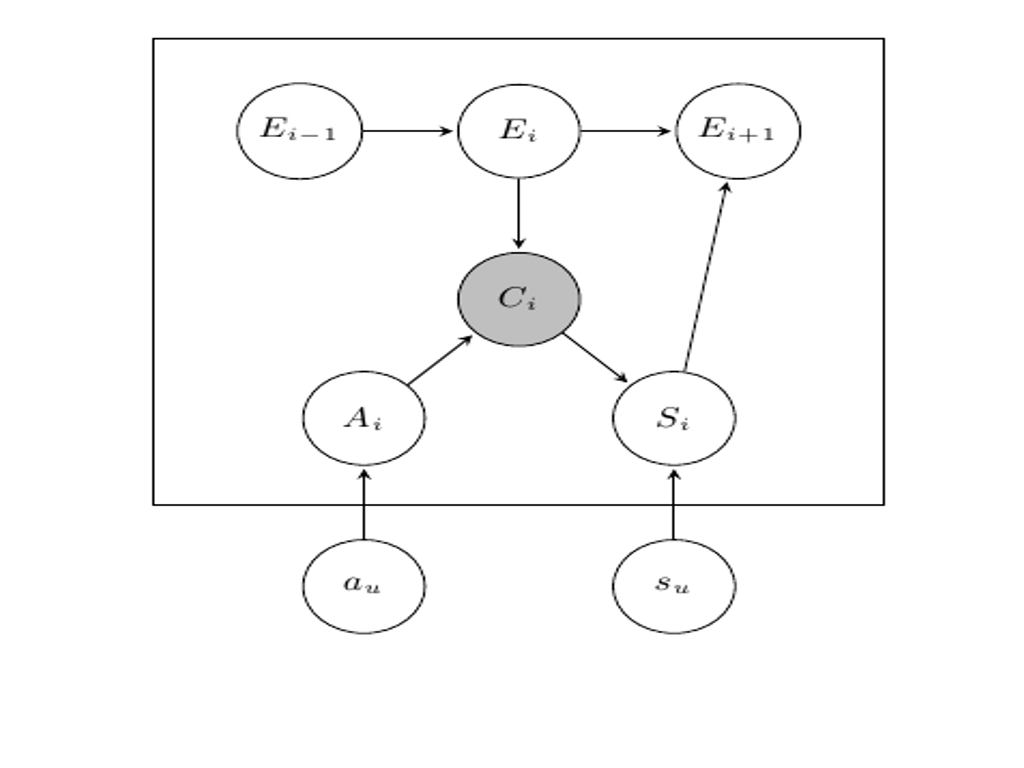
\includegraphics[width=0.9\textwidth]{images/dbn.png}
  \caption{Динамическая байесова сеть\label{dbn-picture}}
\end{figure}

Предполагается, что пользователь произвел клик по документу, если он его исследовал($E_i=1$) и документ его привлек($A_i=1$). Кроме этого, вероятность того, что пользователя привлек документ равняется $a_u$. Также, введен параметр удовлетворенности документом($S_i$). Предполагается, что если пользователь на произвел клик по документу($C_i=0$), то документ был неинформативным($S_i=0$). Иначе, документ считается информативным и пользователь не будет просматривать следующий документ ($S_i=1 \implies E_{i+1}=0$). Если документ оказался неинформативным, то пользователь может с какой-то вероятностью $\gamma$ продолжить сессию $P(E_{i+1}=1|E_i=1,S_i=0)=\gamma$. Т.к. мы предполагаем что данная модель последовательна, то $E_i=0 \implies E_{i+1}=0$.

Определим понятие релевантности документа:
\begin{equation}
	r_u=P(S_i=1|E_i=1)\\
	   =P(S_i=1|C_i=1)P(C_i=1|E_i=1)\\
	   =a_u s_u
\end{equation}


Решение и нахождение релевантности документов зависит от параметра $\gamma$. При $\gamma =1$ нам точно известно, что пользователь остановится после того, как его не удовлетворил документ $i$. Данный алгоритм приведен ниже:

\begin{algorithm}
  \caption{Простой алгоритм нахождения релевантности}
  \label{overall-boosting-algorithm}
  \begin{enumerate}
  \item Инициализировать переменные $a_{u}^{N},a_{u}^{D},s_{u}^{N},s_{u}^{D}$ в значение 0, для всех url ассоциированых для текущего запроса.
  \item Для каждой сессии:
    \begin{enumerate}
      \item Для всех u выше или раано последней кликнутой url в данной сессии:
      	\begin{enumerate}
      		\item $a_{u}^{D}=a_{u}^{D}+1$
      	\end{enumerate}
      \item Для всех url, по которым был произведен клик:
      	\begin{enumerate}
      		\item $a_{u}^{N}=a_{u}^{N}+1$
      		\item $s_{u}^{D}=s_{u}^{D}+1$
      	\end{enumerate}
      \item $s_{u}^{N}=s_{u}^{N}+1$ для последней клинутой url
    \end{enumerate}
    \item для всех url $u$ :
    	\begin{enumerate}
    		\item $a_u=(a_{u}^{N}+\alpha_a)/(a_{u}^{D}+\alpha_a+\beta_a)$
    		\item $s_u=(s_{u}^{N}+\alpha_s)/(s_{u}^{D}+\alpha_s+\beta_s)$
    	\end{enumerate}
  \end{enumerate}
\end{algorithm}

Построение алгоритма EM производится с помощью двух шагов : E и M.
На шаге М, нам даны постериорные распределения скрытых параметров $Q(A_{i}^{j},Q(s_{i}^{j}$. Пересчитываем параметры $a_u,s_u$:

\begin{subequations}
\begin{align}
	a_u=arg \max_a \sum_{j=1}^{N}\sum_{i=1}^{M}I(d_i=u) \nonumber \\
	(Q(A_{i}^{j}=0)\log(1-a)+Q(A_{i}^{j}=1)\log(a))+\log P(a) \\
	s_u=arg \max_s \sum_{j=1}^{N}\sum_{i=1}^{M}I(d_i=u) \nonumber \\
	(Q(S_{i}^{j}=0)\log(1-s)+Q(S_{i}^{j}=1)\log(s))+\log P(s)
\end{align}
\end{subequations}

На шаге Е, по найденным параметрам пересчитываем постериорные вероятности  $Q(A_{i}^{j},Q(s_{i}^{j}$.

\begin{subequations}
\begin{align}
	Q(A_{i}^{j})=P(A_{i}^{j}|C^j,a_u,s_u,\gamma)
	Q(S_{i}^{j})=P(A_{i}^{j}|C^j,a_u,s_u,\gamma)
\end{align}
\end{subequations}

Для ЕМ алгоритма введем дополнительные параметры $\alpha_i(e),\beta_i(e)$:


\begin{subequations}
\begin{align}
	\alpha_i(e)=P(C_{1}^{j},...,C_{i-1}^{j}|E_i=e) \\
	\beta_i(e)=P(C_{i}^{j},...,C_{M}^{j}|E_i=e)
\end{align}
\end{subequations}

Данные параметры мы можем вычислить рекурсивно по правилам:

\begin{subequations}
\begin{align}
	\alpha_{i+1}(e)=\sum_{e \in {0,1}}\alpha_i(e)P(E_{i+1}=e,C_i|E_i=e)\\
	\beta_{i-1}(e)=\sum_{e \in {0,1}}\beta_i(e)P(E_{i}=e,C_{i-1}|E_{i-1}=e)
\end{align}
\end{subequations}

В свою очередь, $P(E_{i+1}=e,C_i|E_i=e)$ вычисляется следующим образом:

\begin{subequations}
\begin{align}
	P(E_{i+1},C_i|E_i)=\sum_{s \in {0,1}}P(E_{i+1}|S_i=s,E_i)P(S_i=s|C_i)P(C_i|E|i)
\end{align}
\end{subequations}

С учетом правил, приведенных выше можно найти релевантности документов. Структура алгоритма ЕМ приведена на ~\ref{em-picture}.

\begin{figure}
  \centering
  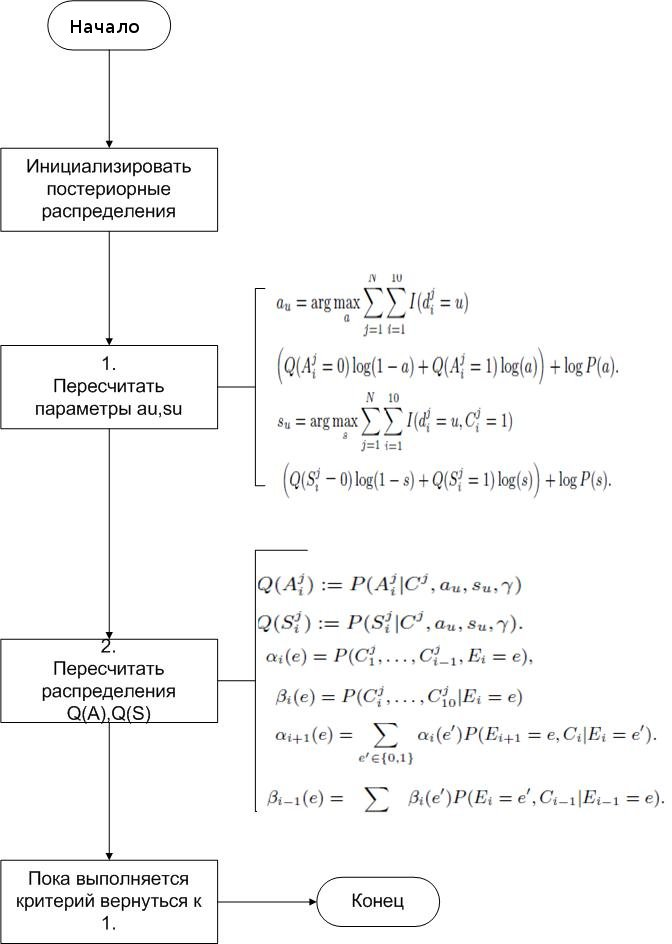
\includegraphics[width=0.9\textwidth]{images/em_new.jpg}
  \caption{Схема ЕМ алгоритма\label{em-picture}}
\end{figure}

\subsection{Выводы}
 
 Данный алгоритм является хорошей опорой для разработки алгоритмов ранжирования. Используемые данные(релевантности документов) будут использованы как конечные цели в тренеровки градиентного бустинга на основе деревьев решений.

К плюсам данного алгоритма можно отнести его относительную легкость построения, быструю сходимость и возможность корректировки результатов с приходом новых данных.

\newpage
\section{Охрана Труда. Безопасность инженеров разработчиков на предприятии малого бизнеса Акавита}

Целью дипломного проекта явилась разработка алгоритмов, которые способствуют улучшению выдачи поисковых систем, путём обучения и анализа поведения пользователей. Техническая суть состоит в создании и разработке алгоритмов которые смогут быть применены на разных типах данных для улучшения релевантности выдачи поисковых систем. Разработка выполнена на предприятии “Акавита”.

В настоящем разделе рассмотрены вопросы, связанные с обеспечением безопасных условий труда инженеров-разработчиков на предприятии малого бизнеса “Акавита”.

Заместителем начальника по управлению кадрами были проведены организационные и инженерно-технические мероприятия по пожарной безопасности. Кроме этого, определен порядок обесточивания электрооборудования по окончании рабочего дня и в случае пожара. Начальник отдела разработки обеспечил пожарную безопасность и противопожарный режим в компании, посредством правильной организации рабочих мест и плана эвакуации. План эвакуации помещения инженеров- 	разработчиков приведен на рисунке ~\ref{evacuation_plan}.

Важную роль в обеспечении пожарной безопасности играет персонал. В компании “Акавита” обучение персонала проводится путем его инструктирования и прохождения пожарно-технического минимума. В связи с законодательством Республики Беларусь ~\cite{ot_1} и приказом директора компании был определен порядок и сроки противопожарного инструктажа и пожарно-технического минимума, а также назначены лица, ответственные за
их проведение. 

\begin{figure}
  \centering
  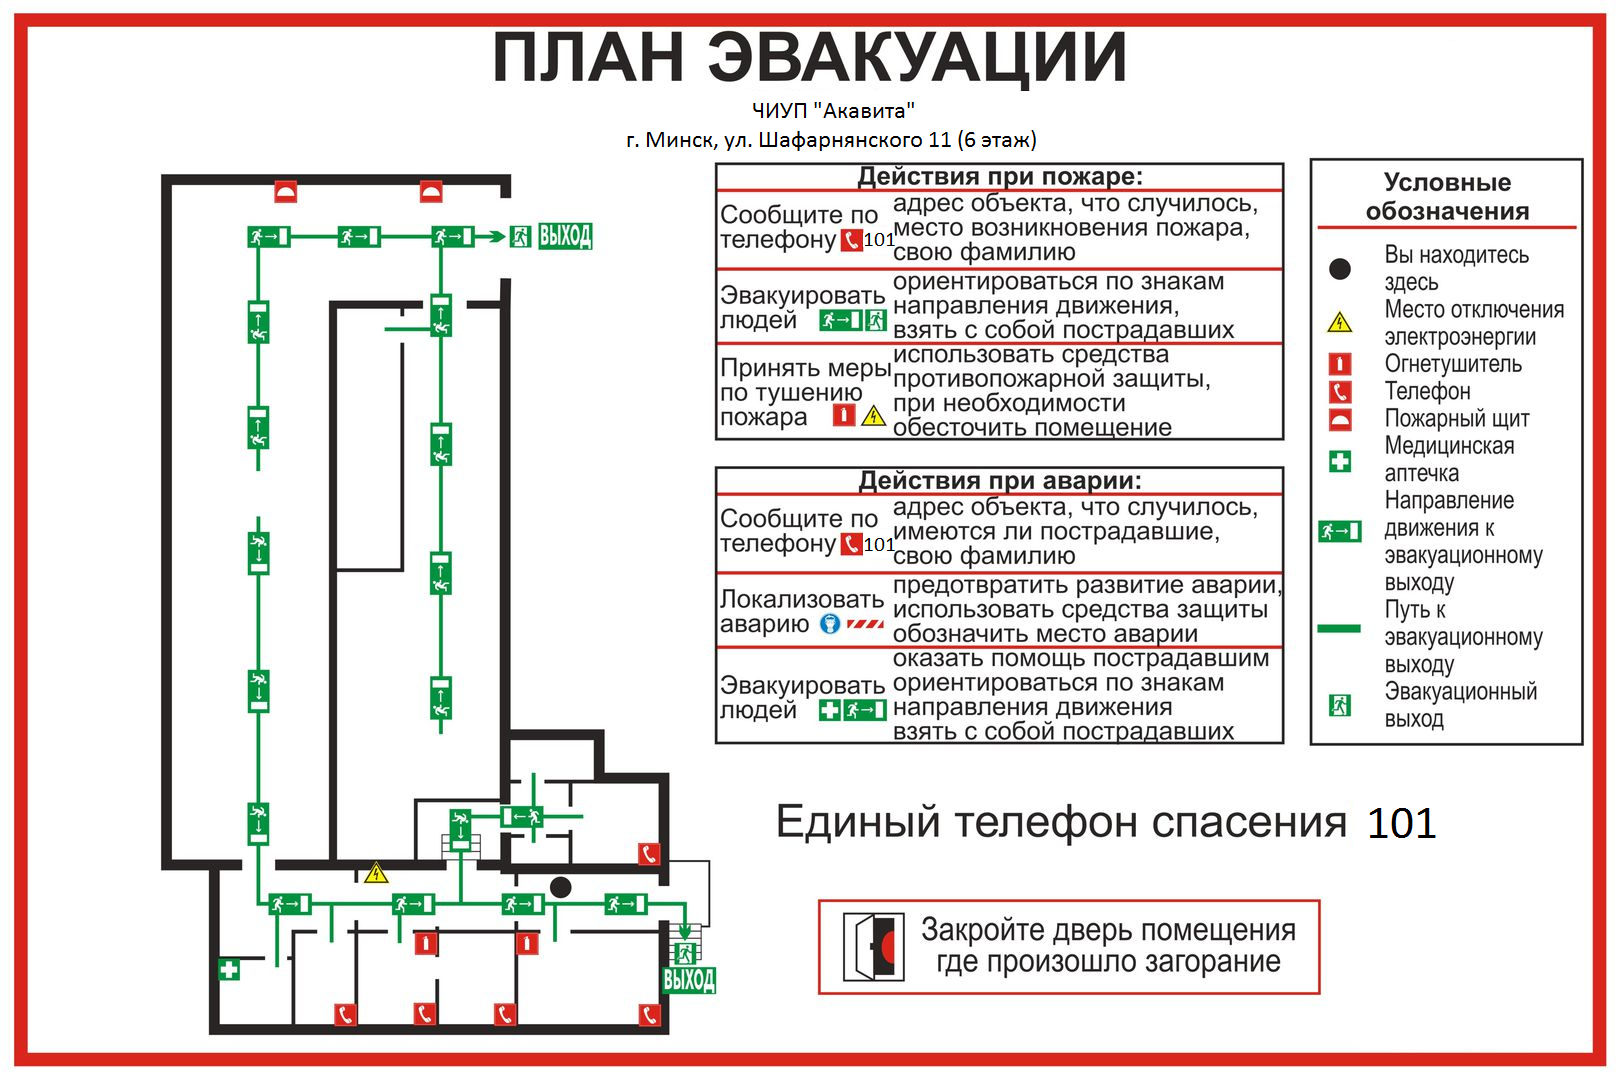
\includegraphics[width=0.9\textwidth]{images/evacuation_plan.png}
  \caption{План Эвакуации разработчиков отдела инженеров-разработчиков в ЧИУП Акавита\label{evacuation_plan}}
\end{figure}

На первичном инструктаже было рассказано об оборудовании, используемом на предприятии, в частности был проведен инструктаж о том, как пользоваться персональным компьютером, принтером, и другим электрическим оборудованием. Были указаны места для курения. Также, были показаны места расположения телефонов и объяснены правила поведения в случае возникновения пожара. 

На предприятии “Акавита” имеются следующие территории: коридор, переговорный зал, игровая комната, отдел разработчиков, отдел тестировщиков, отдел бизнес аналитиков. Для каждого помещения были назначены люди, ответственные за пожарную безопасность этих помещений, а также технологического и инженерного оборудования.

На каждый огнетушитель, установленный на предприятии “Акавита” заведен паспорт. У огнетушителя есть порядковый номер, который нанесен краской на огнетушитель, он записан в эксплуатационный паспорт огнетушителя и в журналы по техническому обслуживанию огнетушителей. Огнетушители размещаются на расстоянии 1.4 м от проёма двери и на высоте 0.2 м.

Чтобы обеспечивалось удобство зрительного наблюдения, быстрое и точное считывание информации, плоскость экрана монитора располагается ниже уровня глаз инженера-разработчика практически перпендикулярно к нормальной линии взгляда работника. Для исключения воздействия повышенных уровней электромагнитных излучений расстояние между экраном монитора и работником составляет не менее 500 мм ~\cite{ot_2}. Рабочий стул (кресло) имеет устойчивое положение, место сидения регулируется по высоте, а спинка сиденья - по высоте, углам наклона, а также расстоянию спинки от переднего края сиденья. Регулировка каждого параметра независима, легко осуществляема и имеет надежную фиксацию. Клавиатура располагается на поверхности стола таким образом, чтобы пространство перед клавиатурой было достаточным для опоры рук инженера-разработчика (на расстоянии не менее чем 350 мм от края, обращенного к работнику ~\cite{ot_2}).

\begin{figure}
  \centering
  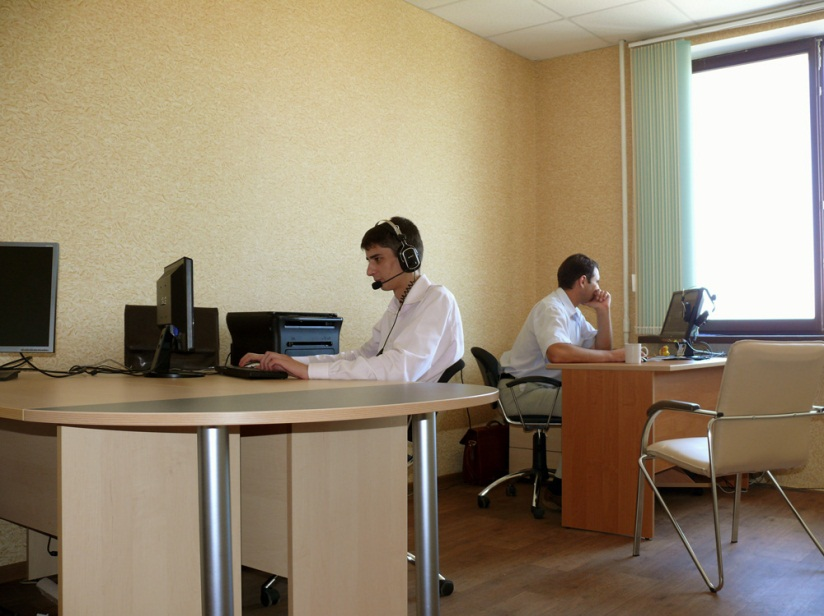
\includegraphics[width=0.9\textwidth]{images/work_place.jpg}
  \caption{рабочее место инженера-разработчика в ЧИУП «Акавита»\label{work_place}}
\end{figure}

Рабочее место размещается таким образом, чтобы естественный свет падал сбоку. Для снижения яркости в поле зрения при естественном освещении применяются регулируемые жалюзи, плотные шторы. Возможные мешающие отражения и отблески на экране монитора и другом оборудовании устраняются путем соответствующего размещения экрана, оборудования, расположения светильников местного освещения. Для обеспечения безопасности инженеров-разработчиков на соседних рабочих местах расстояние между рабочими столами с мониторами составляет 1,5 м, а расстояние между боковыми поверхностями мониторов - 1,4 м ~\cite{ot_2}. Для обеспечения оптимальных параметров микроклимата проводится регулярное в течение рабочего дня проветривание и ежедневная влажная уборка помещений, используются увлажнители воздуха.

При работе с персональным компьютером инженеры-разработчики должны соблюдать режим труда и отдыха, установленный законодательством, правилами внутреннего трудового распорядка организации, трудовую дисциплину, выполнять требования охраны труда, правил личной гигиены. Кроме того, программисты должны выполнять требования пожарной безопасности, знать порядок действий при пожаре, уметь применять первичные средства пожаротушения. Курение производится только в специально предназначенных для курения местах. Особенно важно сообщать о неисправностях оборудования и других замечаниях по работе с персональным компьютером непосредственному руководителю или лицам, осуществляющим техническое обслуживание оборудования. Пример рабочего места в компании «Акавита» приведен на рисунке ~\ref{work_place}.


Таким образом, изложенные выше предложения обеспечат безопасность труда инженеров-разработчиков на предприятии малого бизнеса «Акавита».


\section{Технико экономическое обоснование дипломного проекта}

\subsection{Построение сетевого графика выполнения работ и расчет основных параметров}
\newpage
\setcounter{page}{57}
\subsection{Расчет экономической ээффективности от разработки}

\newpage
\sectioncentered*{Заключение}
\addcontentsline{toc}{section}{Заключение}

Данный дипломный проект демонстрирует построение алгоритма ранжирования использую современные технологии. Была продемонстрирована возможность использования действий пользователей для улучшения ранжирования. Также, централльный алгоритм обучения построен на основе деревьев, что позволяет построить схематический вид и интерпретировать результаты в вид, понятный для людей.
 
В ходе разработки на практике были исследованы возможности построения надежного алгоритма ранжирования на основе бустинга.

Разработанная система полностью удовлетворяет требованиям, сформуливанным в исходных данных к дипломному проекту, и обладает рядом положительных характеристик:
\begin{itemize}
  \item общность, то есть возможность применения данного программного приложения в широком спектре информационного поиска, что существенно отличает задействованный метод от других современных методов,
  \item относительная простота как реализации, так и математической формулировки,
\end{itemize}

Существуют возможности усовершенствования проекта с целью повышения точности и надежности ранжирования результатов. Одним из способов является использование вместе со слабыми классификаторами, такие так нейронная сеть и методы опорных векторов.

Также в будущем планируется опробовать алгоритм градиентного бустинга с регрессионными деревьями. 

В работе было проведено технико-экономическое обоснование разработки системы. Произведенные расчеты показали, что разработка программного обеспечения является рентабельной. Программное обеспечение имеет короткий срок окупаемости.

\newpage
\begin{thebibliography}{99}

\bibitem{joachims}
   Джочим, Т.
  \emph{Оптимизация поисковых систем с использованием кликов данных}./ 
  Т. Джочим // Конференция поисковых технологий --- 2009 -- С. 14-19.

\bibitem{cart_estimation_book}
 Бургес К.
  \emph{Использование бустинга в задаче ранжирования} / Пинг Ли, Кристофер Бургес - М. Вильямс - 2007 г.

\bibitem{cart_optimal3}
  Брамер М.
  \emph{Принципы дата майнинга}. / Макс Брамер --- М. Уолтерс ---  2007 г.

\bibitem{cart_optimal4}
  Горвард Т.
  \emph{Логика. Индуктивное программировани}. / Томас Горвард --- М. Открытые системы - 2003 г.

\bibitem{cart_optimal5}
  Денг Р., Рудгер П.
  \emph{Обобщение важности мер на многозначные атрибуты и их решения}. / Р. Денг, П. Рудгер  М. Физматкнига - 2011 г. 

\bibitem{ctr_improving1}
  Торстен Д. 
  \emph{Оптимизация поисковой программы используя клики данных}. /
  Д. Торстен // 2004 г.

\bibitem{ctr_improving2}
  Эрик Брилл, Сьюзен Димаис
  \emph{Улучшение ранжирования информационного поиска используя поведения пользователей}.
  2006 г.

\bibitem{martin}
  Мартин Дж. К.,
  \emph{Точная вероятностная метрика для расщепления деревьев регения}.
  1997 год. Стр. 257-291.

\bibitem{m_chain}
  Джуди Пирл,
  \emph{Причинность: модели, мышление и вывода}, 2-e изд.
  М.: Издательский дом ``Вильямс'',
  2009.

\bibitem{auc_book}
  Чарльз Линг, Джин Хуанг
  \emph{AUC: Статистически полная и более надежная мера оценки, чем точность измерения}.
  2003 г.

\bibitem{cart_book}
  Data Mining Conferention
  \emph{CART: classification and regression trees}.
  2006 г.

\bibitem{cart_optimal1}
  Хоуфали, Лоурент
  \emph{Построение оптимальных бинарных решающих деревьев является NP полной задачей}.
  2003., стр 15-17.

\bibitem{cart_optimal2}
  Мурфи С.
  \emph{Автоматическое создание решающих деревьев}.
  1998 г.

\bibitem{ccm}
  Том Минка, Майкл Тейлор
  \emph{Последовательная модель кликов}.
  2009 г. 

\bibitem{dbn}
  Оливер Чапеллер, Ya Zhang
  \emph{Использование динамической байесовой сети в задачах информационного поиска}.
  2009 г.

\bibitem{ndcg_book}
  Калевро Джарвелин, Яана Кикалайнен
  \emph{Накопленный прирост на основе оценки информационного посика. }.
  2002., стр 422–446.

\bibitem{cascade_click_book}
  Красвелл Н., Зойтер О.
  \emph{Эксперементальное сравнение моделей кликов, основанных на позициях.}.
  M: ACM, 2006. 87-94

\bibitem{norvig06}
  П. Норвиг, С. Рассел,
  \emph{Искусственный интеллект: современный подход}, 2-е изд.
  М.: Издательский дом ``Вильямс'',
  2006.

\bibitem{ot_1}
  Семенков, В.И.
  \emph{Охрана труда. Сборник нормативных правовых актов.}.
  В.И. Семенков, Липень Л.И. - Минск.: Дикта, 2009 - 784 с.

\bibitem{ot_2}
  [Электронный ресурс].
  \emph{Инструкции по охране труда.}.
  Электронные данные.  – Режим доступа : http://instruction-ot.by

\bibitem{decree432}
  Указ Президента РБ №432 от 31 августа 2009 года,
  \emph{О некоторых вопросах приобретения имущественных прав на результаты научно-технической деятельности и распоряжения этими правами}.
  http://president.gov.by/press76885.html

\bibitem{palitsyn06}
  Палицын В.А.,
  \emph{Технико-экономическое обоснование дипломных проектов. В 4-х частях. Часть 4: проекты программного обеспечения}.
  Мн.: БГУИР,
  2006.

\end{thebibliography}

\newpage


\end{document}

